% -*- coding: UTF-8 -*-
% hurlex-chapt10.tex
% hurlex 开发文档 第10章内容

\section {虚拟内存管理的实现}

\par 这章将详细研讨虚拟内存管理的实现。

\par 上一章谈到,虚拟的页面每页占据4KB,按页为单位进行管理。物理内存也被分页管理,按照4KB分为一个个物理页框。虚拟地址到\allowbreak
物理地址通过由页目录和页表组成的二级页表映射,页目录的地址放置在CR3寄存器里。

\par 至此,我们彻底揭开了x86下32位寻址的面纱,下图描述了地址转换的完整过程。

\begin{figure}[H]
      \centering
      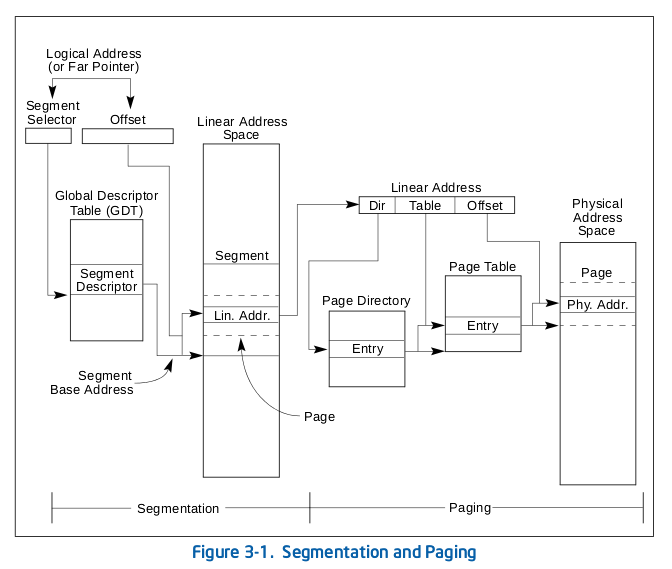
\includegraphics[scale=0.6]{picture/chapt10/ADDR_TRAN.png}
      \caption{段页式转换}
\end{figure}

\par 因为我们使用了Intel平坦模式的内存模型,所以之前的分段机制是被"绕过去"的,所以分页的管理就成了内存管理的核心了。首先是\allowbreak
内核自身地址的映射,Linux采用的是方案是把内核映射到线性地址空间3G以上,而应用程序占据线性地址空间0-3G的位置。我们的内核采取\allowbreak
和Linux内核一样的映射,把物理地址0从虚拟地址0xC0000000(3G)处开始往上映射,因为我们只管理最多512MB的内存,所以3G-4G之间\allowbreak
能完全的映射全部的物理地址。采取这个映射后,物理地址和内核虚拟地址满足以下关系:

\par 物理地址 + 0xC0000000 = 内核虚拟地址

\par 但是采用这个设计的话会给我们已有的代码带来什么麻烦呢?

\par 首先是链接器,我们需要修改链接器脚本中各个段的起始位置。但是简单的把代码段的起始位置设为0xC0100000的话内核一运行就出错。\allowbreak
为什么呢?因为GRUB是从1MB处加载内核的,而链接器是以0xC0100000这个参考地址进行地址重定位的。此时尚未开启虚拟页面映射,运行\allowbreak
寻址的代码肯定就会出错。怎么办呢?看起来像是一个无解的死循环了。如果GRUB在加载内核之前就能设定好虚拟地址的映射再执行内核\allowbreak
多好,或者有一段程序和数据按照0x100000的地址进行重定位,能帮助我们设置好一个临时的页表,再跳转到内核入口函数多好。前者\allowbreak
貌似不可能实现,那后者呢?答案是肯定的,我们就采用这个方案。

\par GCC提供了这样的扩展机制:允许程序员指定某个函数或者某个变量所存储的区段。同时ld的链接脚本又可以自由定制,所以这个\allowbreak
无解的问题就有了解决方案。用于设置这个临时页表和函数我们指定它存储在.init段,只需要指定该段从0x100000地址开始,\allowbreak
其他的.text和.data等段按照0xC0100000作为起始地址即可。当然这里还有要注意的细节,具体在下面的新链接脚本中可以看到:


\par



\par 另外还需要修改文本模式下显存的起始位置,原先的地址0xB8000此时需要加上偏移地址0xC0000000才可以在分页模式下正常访问到。
